\chapter{Why You Need To Learn Sales Before You Start a Company}

This chapter is built from a short interview answer, not from a blackboard derivation, but it still has a precise internal logic. The opening claim is severe: experience is not searchable information. It is something we pass through. The rest of the discussion explains how early sales work becomes a training ground for company-building by exposing us to rejection, forcing us to keep our composure, and teaching us to deliver the same message to many kinds of people. To make that mechanism easier to see, we will use a light notation throughout, always as an editorial summary of the transcript rather than as speaker-given formalism.

\section{Experience Cannot Be Googled}

The first sentence gives the answer before the question is fully stated. That is the right place to begin. We are told, in effect, that there is a difference between information that can be retrieved and experience that can only be lived. If we want a compact way to write that distinction, we may say
\begin{equation}
E_{\mathrm{lived}} \neq E_{\mathrm{textbook}}.
\end{equation}
Here \(E_{\mathrm{lived}}\) denotes direct passage through real encounters, while \(E_{\mathrm{textbook}}\) denotes secondhand instruction, reading, and advice.

The point is not that advice is worthless. The point is narrower and sharper. There is a class of entrepreneurial competence that does not transfer merely by description. The lecture begins by drawing that boundary with unusual force, and the rest of the chapter should be read inside that boundary.

\section{From Sales to Ownership}

Only after the opening claim do we hear the explicit frame: early in his career, the speaker worked primarily in sales, and the question is how that experience translated into owning a company at a young age. The answer is not presented as a list of tactics. It is presented as a mechanism of formation.

\begin{definition}
We introduce the following working symbols:
\begin{align}
T &:= \{\text{tricks},\ \text{phrases},\ \text{appearance}\}, \\
S &:= \text{practical sales skill}, \\
N &:= \text{repeated negative encounters}, \\
A &:= \text{attitude stability under pressure}, \\
M &:= \text{message delivery under pressure}, \\
V &:= \text{audience variation}.
\end{align}
These symbols are not quoted from the source; they are a compact way to preserve its causal structure.
\end{definition}

The entrepreneurial question is therefore not merely, ``What did sales teach him?'' It is, more exactly, ``What kind of thing does sales teach that later becomes useful in building and leading a company?'' The lecture answers by separating surface instruction from embodied competence.

\section{What Can Be Taught, and What Cannot}

The speaker concedes an important point at once. Someone can teach the tricks. Someone can teach the cool things to say. One can even learn to present oneself well. In our shorthand,
\begin{equation}
T = \{\text{tricks},\ \text{phrases},\ \text{appearance}\}.
\end{equation}
But the argument is that this does not yet amount to real selling skill:
\begin{equation}
S \neq T.
\end{equation}

This concession matters. Without it, the claim that ``no textbook can teach it'' would sound too broad. The lecture is more careful than that. It grants the limited truth of instruction and then denies its sufficiency. Sales, in the strong sense intended here, is not just possession of lines or polish. It is the ability to remain effective when those surface tools are placed under stress.

\subsection{Question \& Answer}

Why does a textbook fail here, even if it gives us useful phrases and useful advice?

Because the decisive part of the skill is not the possession of verbal material but the use of that material under adverse conditions. In the transcript, the answer comes through a sequence of tests: being told no, being cursed at, being screamed at, and still needing to keep the same attitude while delivering the message the right way. That is why the lecture can be summarized by the directional statement
\begin{equation}
E_{\mathrm{textbook}} \not\to S,
\qquad
E_{\mathrm{lived}} \to S.
\end{equation}
The arrow here is causal, not mathematical in a strict sense. The point is simply that lived exposure produces a kind of competence that description alone does not.

\section{Rejection as Training}

Now we come to the real center of the lecture. The speaker does not mention adversity once and move on. He stacks it: no, then more no, then hostility, then the demand that the salesperson continue to show the same attitude and deliver the message correctly. This is the mechanism, and it deserves to be written in a way that preserves its sequence.

Let \(R_k\) denote the \(k\)-th live encounter. A cautious update rule, used only as shorthand for the transcript, is
\begin{align}
S_{k+1} &= S_k + \Delta S_k, \\
\Delta S_k &= h(R_k, A_k, M_k, V_k).
\end{align}
The intended reading is simple. A live encounter changes us. If the encounter includes resistance, and if we manage to hold our attitude together while still delivering the message, then there is room for a gain in skill.

A worked version of the argument is as follows.
\begin{enumerate}
\item We begin with surface preparation \(T\): what to say, how to dress, how to present.
\item We then enter a live encounter \(R_k\), where the other person may reject us outright.
\item That encounter raises the practical demand to maintain \(A_k\), the same attitude, under pressure.
\item At the same time, it raises the practical demand to maintain \(M_k\), the right delivery of the message.
\item If both demands are met well enough, then \(\Delta S_k > 0\): the next attempt is made by a more seasoned agent than the previous one.
\end{enumerate}

The lecture does not quantify these increments, and we should not pretend that it does. Still, the update form is useful because it keeps the logic of repetition visible. Skill is not transferred all at once. It is accumulated through encounter after encounter.

\begin{figure}[h]
\centering
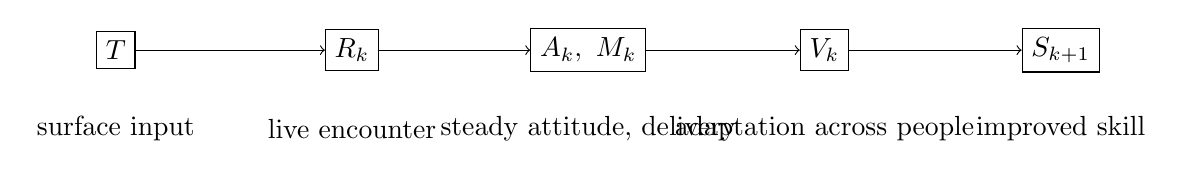
\begin{tikzpicture}
\node[draw, rectangle] (t) at (0,0) {$T$};
\node[draw, rectangle] (r) at (3,0) {$R_k$};
\node[draw, rectangle] (am) at (6,0) {$A_k,\ M_k$};
\node[draw, rectangle] (v) at (9,0) {$V_k$};
\node[draw, rectangle] (s) at (12,0) {$S_{k+1}$};

\draw[->] (t) -- (r);
\draw[->] (r) -- (am);
\draw[->] (am) -- (v);
\draw[->] (v) -- (s);

\node at (0,-1) {surface input};
\node at (3,-1) {live encounter};
\node at (6,-1) {steady attitude, delivery};
\node at (9,-1) {adaptation across people};
\node at (12,-1) {improved skill};
\end{tikzpicture}
\end{figure}

The figure is not a recovered lecture graphic. It is a clean summary of the causal flow that the transcript itself unfolds in time.

\section{Learning Across Difference}

After the rejection sequence, the lecture adds one more ingredient. Sales does not merely expose us to pressure. It exposes us to variety: different ethnicities, different backgrounds, different ages, different experiences. The effect of this addition is to prevent us from imagining that skill consists in surviving one kind of difficult interaction. Instead, it consists in learning to communicate across many forms of human difference.

That is why a useful summary is
\begin{equation}
S = f(N, A, M, V).
\end{equation}
Here \(N\) measures repetition of negative encounters, \(A\) measures stability of attitude, \(M\) measures the quality of message delivery, and \(V\) measures the range of audiences one must learn to address. The point is not that the speaker offers a formula. The point is that the transcript clearly identifies these as the active ingredients in improvement.

The concluding causal claim can then be written as
\begin{equation}
N \uparrow,\ V \uparrow \quad \Longrightarrow \quad S \uparrow,
\end{equation}
provided that the salesperson continues to hold together the two practical constraints already emphasized: the same attitude and the right delivery. This is the meaning of the final sentence that under these conditions one has no choice but to get better.

We should notice how strong that closing claim is. Improvement is not presented as a matter of inspiration or mood. It is presented as the natural consequence of repeated live contact with resistance and variety. The entrepreneurial payoff is then easy to see. A founder who has survived this kind of training is harder to rattle, more adaptable in communication, and better prepared to lead.

\section{Summary}

The argument of the lecture is short, but it is tightly organized. First, experience is separated from searchable information. Second, the entrepreneurial frame is supplied: we are asked how sales translates into company ownership. Third, the speaker grants that some things can be taught, but insists that these things do not yet amount to real skill. Fourth, the transcript identifies the true training mechanism: repeated rejection, stable attitude, correct delivery. Finally, it broadens the field from pressure alone to pressure across many kinds of people, and concludes that under such conditions improvement is nearly unavoidable.

If we keep the order of these moves intact, we preserve the real rhythm of the source. Sales matters here not as a bag of tactics but as a school of exposure. That is the practical theorem of the chapter: the person who has had to pass through repeated live resistance is prepared, in a deeper way, for the work of building a company.